Det følgende er et diagram over find_best funktion:
\begin{figure}[!h]
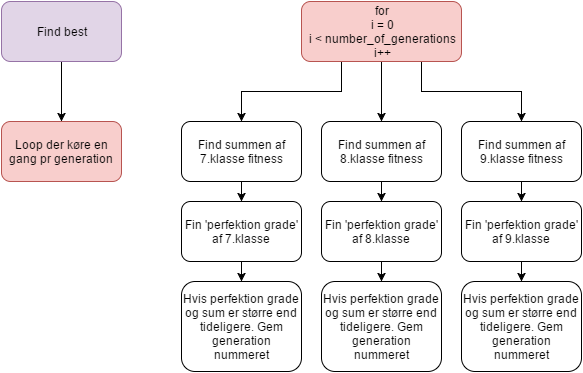
\includegraphics[width=\textwidth]{partials/graphics/bestof.png}
\caption{Grafisk diagram over find_best funktionen}
\label{fig:diagrambestof}
\end{figure}

De forskellige klassetrin bliver beregnet for sig, uden at kunne påvirke hinanden. For at finde det bedste skema der er blevet generet for hver klassetrin, på tværs af generationer, bliver alle de bedste skemaer for de enkelte generationer gået gennem, og der bliver udvalgt tre generationer. Den med den bedste 7. klasse, den bedste 8. klasse og den bedste 9. klasse. Disse bliver nu sat sammen til deres eget individ, som bliver printet i print funktionen. 

\begin{lstlisting}[language=c]

void find_best(individual chosen_individuals[][NUMBER_OF_GENERATIONS], individual best_of_best[]){
  printf("\n\n");
  int i, k, j = 0;
  int best_sum1, best_sum2, best_sum3;
  int best_gen1, best_gen2, best_gen3;
  int sum1, sum2, sum3;
  int temp_perfect1 = 0, temp_perfect2 = 0, temp_perfect3 = 0;
  int perfect1 = 0, perfect2 = 0, perfect3 = 0;
  
  for (i = 0; i < NUMBER_OF_GENERATIONS; i++){
    /* Getting the sum */
    if ((chosen_individuals[0][i].fitness != 1) && (chosen_individuals[1][i].fitness != 1) && (chosen_individuals[2][i].fitness != 1)){
      sum1 = chosen_individuals[0][i].fitness + chosen_individuals[1][i].fitness + chosen_individuals[2][i].fitness;
    }
    else {
      sum1 = 0;
    }

    if ((chosen_individuals[3][i].fitness != 1) && (chosen_individuals[4][i].fitness != 1) && (chosen_individuals[5][i].fitness != 1)){
      sum2 = chosen_individuals[3][i].fitness + chosen_individuals[4][i].fitness + chosen_individuals[5][i].fitness;
    }
    else {
      sum2 = 0;
    }

    if ((chosen_individuals[6][i].fitness != 1) && (chosen_individuals[7][i].fitness != 1) && (chosen_individuals[8][i].fitness != 1)){
      sum3 = chosen_individuals[6][i].fitness + chosen_individuals[7][i].fitness + chosen_individuals[8][i].fitness;
    }
    else {
      sum3 = 0;
    }

    /* Getting the lowest perfection grade */
    temp_perfect1 = 15;
    temp_perfect2 = 15;
    temp_perfect3 = 15;

    if (temp_perfect1 > chosen_individuals[0][i].perfection){
      temp_perfect1 = chosen_individuals[0][i].perfection;
    }
    if (temp_perfect1 > chosen_individuals[1][i].perfection){
      temp_perfect1 = chosen_individuals[1][i].perfection;
    }
    if (temp_perfect1 > chosen_individuals[2][i].perfection){
      temp_perfect1 = chosen_individuals[2][i].perfection;
    }

    if (temp_perfect2 > chosen_individuals[3][i].perfection){
      temp_perfect2 = chosen_individuals[3][i].perfection;
    }
    if (temp_perfect2 > chosen_individuals[4][i].perfection){
      temp_perfect2 = chosen_individuals[4][i].perfection;
    }
    if (temp_perfect2 > chosen_individuals[5][i].perfection){
      temp_perfect2 = chosen_individuals[5][i].perfection;
    }

    if (temp_perfect3 > chosen_individuals[6][i].perfection){
      temp_perfect3 = chosen_individuals[6][i].perfection;
    }
    if (temp_perfect3 > chosen_individuals[7][i].perfection){
      temp_perfect3 = chosen_individuals[7][i].perfection;
    }
    if (temp_perfect3 > chosen_individuals[8][i].perfection){
      temp_perfect3 = chosen_individuals[8][i].perfection;
    }

    /* Saving the best */
    if (perfect1 < temp_perfect1){
      best_sum1 = sum1;
      best_gen1 = i;
      perfect1 = temp_perfect1;
      printf("  1  perfection: %d  sum: %d \n", perfect1, best_sum1);
    }
    else if (perfect1 == temp_perfect1){
      if (best_sum1 < sum1){
        best_sum1 = sum1;
        best_gen1 = i;
        perfect1 = temp_perfect1;
        printf("  1  perfection: %d  sum: %d \n", perfect1, best_sum1);
      }
    }

    if (perfect2 < temp_perfect2){
      best_sum2 = sum2;
      best_gen2 = i;
      perfect2 = temp_perfect2;
      printf("  2  perfection: %d  sum: %d \n", perfect2, best_sum2);
    }
    else if (perfect2 == temp_perfect2){
      if (best_sum2 < sum2){
        best_sum2 = sum2;
        best_gen2 = i;
        perfect2 = temp_perfect2;
        printf("  2  perfection: %d  sum: %d \n", perfect2, best_sum2);
      }
    }

    if (perfect3 < temp_perfect3){
      best_sum3 = sum3;
      best_gen3 = i;
      perfect3 = temp_perfect3;
      printf("  3  perfection: %d  sum: %d \n", perfect3, best_sum3);
    }
    else if (perfect3 == temp_perfect3){
      if (best_sum3 < sum3){
        best_sum3 = sum3;
        best_gen3 = i;
        perfect3 = temp_perfect3;
        printf("  3  perfection: %d  sum: %d \n", perfect3, best_sum3);
      }
    }
  }
  
  best_of_best[0] = chosen_individuals[0][best_gen1];
  best_of_best[1] = chosen_individuals[1][best_gen1];
  best_of_best[2] = chosen_individuals[2][best_gen1];
  best_of_best[3] = chosen_individuals[3][best_gen2];
  best_of_best[4] = chosen_individuals[4][best_gen2];
  best_of_best[5] = chosen_individuals[5][best_gen2];
  best_of_best[6] = chosen_individuals[6][best_gen3];
  best_of_best[7] = chosen_individuals[7][best_gen3];
  best_of_best[8] = chosen_individuals[8][best_gen3];
  
  for (j = 0; j < NUMBER_OF_CLASSES; j++){
    best_of_best[j].best_gena7 = best_gen1;
    best_of_best[j].best_gena8 = best_gen2;
    best_of_best[j].best_gena9 = best_gen3;
  }
  printf("\n\n");
  printf("  1  perfection: %d  sum: %d \n", perfect1, best_sum1);
  printf("  2  perfection: %d  sum: %d \n", perfect2, best_sum2);
  printf("  3  perfection: %d  sum: %d \n\n", perfect3, best_sum3);
}

\end{lstlisting}

Denne funktion tager ’chosen\_individuals[][]’ og ’best\_of\_best[]’ som parametre. En for lykke kører en gang for hver generation der er. I lykken er der nogle if-sætninger, hvis formål er at finde summen for parallelklasserne samt finde den parallel klasse som har den laveste ’perfektion-grade’. Dette gør den da, den leder efter den generation, hvor en bestemt klasse har den højeste perfektion-grade, og den højeste sum. Dog skal programmet først og fremmest, finde den klasse med den bedste perfektion grade. 
Derfor tjekkes der nu med if-sætninger, om perfektion-grade er bedre end den tidligere bedste. Hvis den nuværende generation er bedre end de forrige. Blive denne nu gemt.